\documentclass[pdf]{beamer}

\usepackage[utf8]{inputenc}
\usepackage[brazil]{babel}
\usepackage{graphicx}
\usepackage[normalem]{ulem}
\usepackage{listings}
\usepackage{hyperref}

\hypersetup{colorlinks=true,linkcolor=blue,urlcolor=blue,citecolor=blue,anchorcolor=blue}

\lstset{breakatwhitespace,
  language=C,
  columns=fullflexible,
  keepspaces,
  breaklines,
  tabsize=4,
  showstringspaces=false,
  extendedchars=true,
  keywordstyle=\color{blue}\ttfamily,
  stringstyle=\color{red}\ttfamily,
  commentstyle=\color{green!40!black}\ttfamily,
  morecomment=[l][\color{magenta}]{\#}
}

\lstset{breakatwhitespace,
  language=Python,
  columns=fullflexible,
  keepspaces,
  breaklines,
  tabsize=4,
  showstringspaces=false,
  extendedchars=true,
  keywordstyle=\color{blue}\ttfamily,
  stringstyle=\color{red}\ttfamily,
  commentstyle=\color{green!40!black}\ttfamily,
  morecomment=[l][\color{magenta}]{\#}
}

%\usetheme{progressbar}

\title[Outreachy]{Applying for Outreachy}

\author{{\Large Wander Lairson Costa}}
\institute{{\large Mozilla Corporation}}

\date{}

\begin{document}

\begin{frame}
  \titlepage
  \begin{center}
    \begin{tabular}{c}
      \url{https://twitter.com/walac00} \\
      \url{https://www.facebook.com/wander.costa} \\
      \url{https://github.com/walac} \\
      \href{mailto:wcosta@mozilla.com}{wcosta@mozilla.com}
    \end{tabular}
  \end{center}
\end{frame}

\begin{frame}{What is it}
  \begin{itemize}
    \item A program for under represented groups
    \item Evolution of Outreachy Program for Women
    \item \$5500 USD for 3 month remote internship
    \item \$500 USD for travel allowance
  \end{itemize}

  More info: \url{https://wiki.gnome.org/Outreachy}
\end{frame}

\begin{frame}{Eligible people}
  People who don't live of in any of the following countries:
  \vspace{1em}
  \begin{minipage}{.45\linewidth}
    \begin{itemize}
        \item Crimea
        \item Cuba
        \item Iran
    \end{itemize}
  \end{minipage}
  \hspace{.05\linewidth}
  \begin{minipage}{.45\linewidth}
    \begin{itemize}
        \item North Korea
        \item Syria
        \item Sudan
    \end{itemize}
  \end{minipage}

  \vspace{1em}
  And identify themselves as:
  \begin{itemize}
    \item Women (cis or trans)
    \item Trans men
    \item Genderqueers
    \item People of color living in USA
  \end{itemize}

  \begin{center}
    \begin{minipage}{.45\linewidth}
      \begin{itemize}
        \item Afro-american
        \item American indian
        \item Alaska Native
      \end{itemize}
    \end{minipage}
    \hspace{.05\linewidth}
    \begin{minipage}{.45\linewidth}
      \begin{itemize}
        \item Native Hawaiian
        \item Pacific Islander
        \item Hispanic/Latin
      \end{itemize}
    \end{minipage}
  \end{center}
\end{frame}

\begin{frame}{General steps}
  You must have 40 hours/week available for internship

  \begin{enumerate}
    \item Get in touch with mentor for the project you are applying to
    \item Join \#outreachy IRC channel at \url{irc.gnome.org}
    \item Subscribe to \url{mailto:outreachy-list@gnome.org}
    \item Make a contribution
    \item Apply at \url{https://outreachy.gnome.org}
  \end{enumerate}
\end{frame}

\begin{frame}{Mozilla specific}
  \begin{itemize}
    \item \#outreachy IRC channel at \url{irc.mozilla.org}
    \item Outreachy wiki page \url{https://wiki.mozilla.org/Outreachy}
    \item Interns join Mozilla All Hands
  \end{itemize}

  \begin{center}
    Larissa Shapiro \href{mailto:lshapiro@mozilla.com}{lshapiro@mozilla.com}
    Diversity and Inclusion Programs Manager
  \end{center}
\end{frame}

\begin{frame}{Tips}
  \begin{itemize}
    \item Talk to project mentor either by IRC or email about first contribution
    \item Don't be affraid of asking questions
    \item Don't pick the easiest patch
    \item Apply early and apply for more than one project
    \item If you can, make more than one contribution
    \item \url{http://outreachy.anaplusplus.com/2016/05/what-is-outreachy-and-how-to-apply-for.html}
  \end{itemize}
\end{frame}

\begin{frame}{Questions}
  \begin{center}
    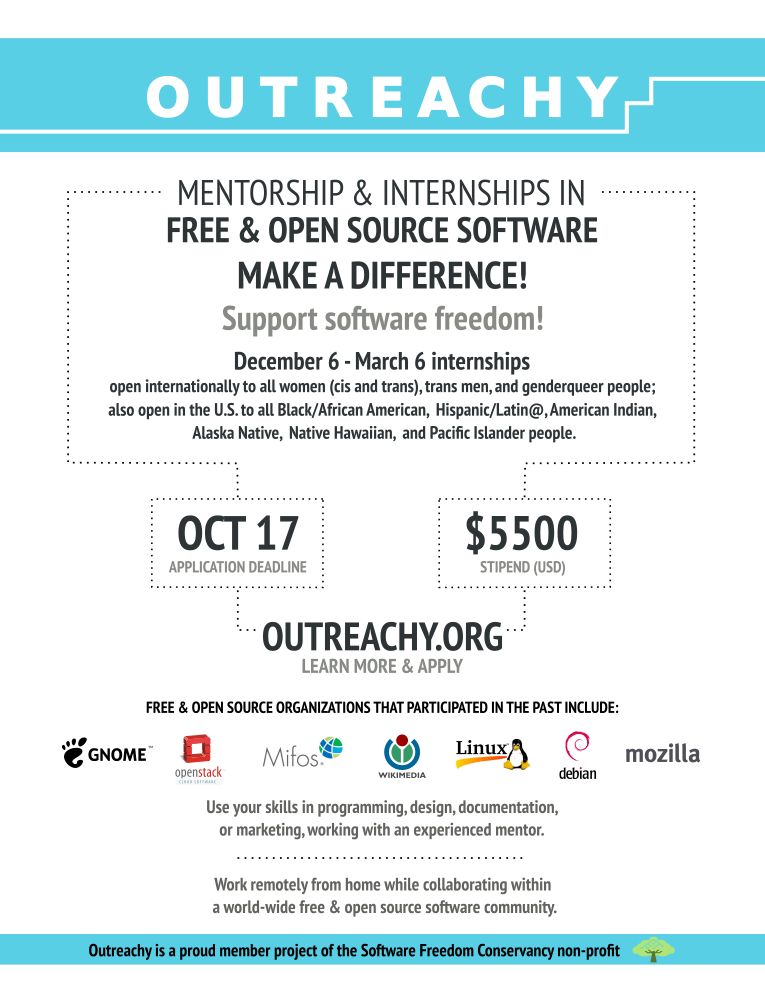
\includegraphics[scale=0.3]{img/outreachy-applicants-2016-December.png}
  \end{center}
\end{frame}

\end{document}

